\section{Coupling through preCICE}
When a physical problem becomes too complex, one often split it into smaller pieces that are better manageable. These pieces, or physical fields, can then be solved separately and their solutions can be combined to an overall solution. This approach is called ``partitioned approach'' \cite{gatzhammer2015efficient}. This approach allows to reuse the simulation code for the single fields and simultaneously provides the possibility to encapsulate the coupling functionality itself as a reusable component, too. This allows minimal access to solver codes, i.e., treating them as black boxes. At the same time the solver code does not have to include the whole coupling code making it less application dependent. The coupling tool preCICE offers coupling functionality to develop a multi-physics simulation environment using existing solvers. In this work a fluid-structure interaction (FSI) will be simulated. The thesis' program represents the structure part whereas the fluid part can be dynamically exchanged due to the coupling with preCICE. This Chapter gives an overview of preCICE and its main components and shows the implementation modifications that were necessary to integrate preCICE and prepare the code for coupling.

 \subsection{Overview of preCICE} %gelbe Marker
  The goal of preCICE is to provide all functionality to realize a multi-physics simulation environment working with existing single-physics solvers. This includes simulations like fluid-structure, fluid-acoustics, fluid-solid thermodynamics and porous-free flow interactions, for instance. It provides technical inter-code communication via MPI or TCP/IP, methods for data mapping between different grids and coupling methods based on quasi-Newton methods to ease the development process. preCICE supports parallel solvers through efficient point-to-point communication without the need of a server instance. It also features a high-level API making its integration into existing solver code minimal invasive \cite{bungartz2015fully}.
  
  preCICE supports partitioned coupling of black box solvers with focus on FSI and provides a geometry interface for Cartesian grid solvers. Its API is available for C++, C, and Fortran and consists of high-level methods enabling solvers to use coupling functionality in a flexible way. After the preCICE integration into the solver's code, a peer-to-peer communication without central control instance is generated. The single solver codes can be run serial or parallel without major modifications to the integrated API. Furthermore, the concrete coupling algorithms in the simulation can be selected through an XML configuration file that optimizes the solver adaption \cite{gatzhammer2015efficient}.
  
  \begin{figure}[htbp]
  	\centering
  	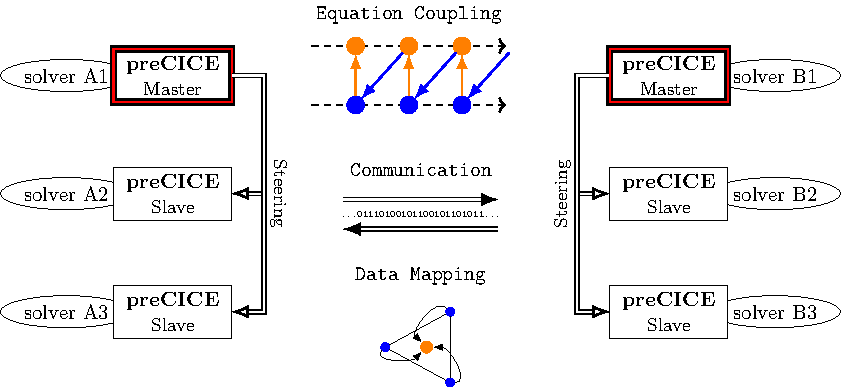
\includegraphics[width=0.97\linewidth]{figures/NewCommunicationScheme}
  	\caption{Schematic view of a partitioned multi-physics simulation with two solvers (A and B) coupled through preCICE. In the middle are the three main functionalities of preCICE shown, that steer coupling iterations: Fix-point acceleration methods, point-to-point communication and data mapping between non-matching grids at the coupling interface. Picture courtesy of Florian Lindner \cite{bungartz2015fully} }
  	\label{fig:precice}
  \end{figure}
  
  Figure \ref{fig:precice} shows a schematic view of the main functionality groups of preCICE. Two solvers (A and B) are coupled through the preCICE tool. The three main functionalities of preCICE are drawn in the middle: Fix-point acceleration methods, point-to-point solver process communication and data mapping between non-matching grids at the coupling surface. Each shown solver runs in parallel with a master process controlling tasks such as convergence for the corresponding solver as well as for the whole simulation. The following sections describe each of the three addressed main functionalities in greater detail.
  
 
 \subsection{Coupling methods} % türkise Marker
 
  \subsubsection{Explicit Coupling Schemes}
  
  \subsubsection{Implicit Coupling Schemes}
  
  \subsubsection{Quasi-Newton approaches}

  

 \subsection{Data Mapping} % rosa Marker

  \subsubsection{Nearest-Neighbor}
  
  \subsubsection{Nearest-Projection}
  
  \subsubsection{Radial Basis Function}



 \subsection{Communication} % hellblaue Marker
  The coupling of different solvers in the frame of a multi-physics simulation requires an efficient communication between different executables. preCICE offers a communication per interaction of two or more participants. Either MPI ports or low level TCP/IP sockets are available for communication in preCICE. A fully parallel point-to-point data transfer is possible with preCICE, since it analyses the mesh decomposition of all participants and constructs only local communication channels where they are needed \cite{bungartz2015fully}.
 
  \subsubsection{MPI Communication}
   The message passing interface (MPI) is used in preCICE with a multiple program multiple data paradigm, i.e. two different codes are communicating with their own data. Two MPI-based communication methods are implemented which differ in the way how they set up the communication space. With the first method all executables are put in the same communication space, called ``communicator world''. All processes of each participant are then grouped into separate communicators. An inter-communicator is used as the actual channel for data exchange.
   The second method establishes a connection between processes started individually and in different communication spaces. The exchange of connection information is done through a commonly accessible file which stores the port names of the participants. For this a MPI version of 2 or greater is needed \cite{gatzhammer2015efficient}. The result is the same as with method one: An inter-communicator.
   
  \subsubsection{Socket Communication}
   The communication by TCP/IP increases compatibility to closed-source software that might be restricted to some MPI implementations \cite{bungartz2015fully}. To abstract from platform dependent socket interfaces like Pthreads or Winsock, the Boost.Asio (asynchronous network and low-level input/output) library was used for implementing the socket communication in preCICE \cite{gatzhammer2015efficient}. The sending and receiving of data is managed by the transfer control protocol (TCP) which is designed for failsafe data transfer and synchronization between sender and receiver. Communication via TCP is not typical for multi-physics simulations that often run on supercomputers, because it involves a synchronization step and additional communication overhead compared to MPI. Other difficulties are that ports used for socket communication may be blocked by default and each supercomputer node might have different network address which requires automated checks on a low-level socket layer \cite{gatzhammer2015efficient}.


 \subsection{Implementation}
 % TODO: text
 
  \subsubsection{Additional Boundary Conditions}
   \begin{itemize}
  	\item - 2: inner node, part of preCICE interface region (only used by preCICE coupled variant)\\
  	- 20: same as 0 but additionally part of preCICE interface region (only used...)\\
  	- 21: same as 1 but additionally part of preCICE ...
  	\end{itemize}
  
  	
  \subsubsection{Partitioned Coupling Surface}
   the surface interface between the solvers is partitioned across the mpi processes of the structure solver. every process needs to construct a grid for itself
   
   
  \subsubsection{Integration of preCICE}
   the main-function gets modified with the preCICE code
 
\newpage